%%%%%%%%%%%%%%%%%%%%%%%%%%%%%%%%%%%%%%%%%%%%%%%%%%%%%%%%%%%%%%%%%%%%%%%%%%%%%%%%
%2345678901234567890123456789012345678901234567890123456789012345678901234567890
%        1         2         3         4         5         6         7         8

\documentclass[letterpaper, 10 pt, conference]{ieeeconf}  % Comment this line out if you need a4paper

%\documentclass[a4paper, 10pt, conference]{ieeeconf}      % Use this line for a4 paper

\IEEEoverridecommandlockouts                              % This command is only needed if 
                                                          % you want to use the \thanks command

\overrideIEEEmargins                                      % Needed to meet printer requirements.

% See the \addtolength command later in the file to balance the column lengths
% on the last page of the document

% The following packages can be found on http:\\www.ctan.org
%\usepackage{graphics} % for pdf, bitmapped graphics files
%\usepackage{epsfig} % for postscript graphics files
%\usepackage{mathptmx} % assumes new font selection scheme installed
%\usepackage{times} % assumes new font selection scheme installed
\usepackage{amsmath} % assumes amsmath package installed
\usepackage{amssymb}  % assumes amsmath package installed
\usepackage{accents}
\usepackage{graphicx}
\newcommand\ubar[1]{%
	\underaccent{\bar}{#1}}
\usepackage{framed}
\usepackage{cite}

\title{\LARGE \bf
Energy Efficient Explosive Motion with Compliant Actuation Arrangements in Articulated Robots
}


\author{Roel Djajadiningrat$^{1}$, Wesley Roozing$^{2}$ and Nikolaos G. Tsagarakis$^{2}$% <-this % stops a space
\thanks{$^{1}$ Roel Djajadiningrat is a M.Sc student at the Department of Mechanical Engineering, TU Delft and a visiting student at Istituto Italiano di Tecnologia;
        {\tt\ r.djajadiningrat@student.tudelft.nl}
  }%
\thanks{$^{2}$Wesley Roozing and Nikolaos G. Tsagarakis are with the Department of Advanced Robotics,
	(Fondazione) Istituto Italiano di Tecnologia, via Morego,
	30, 16163 Genova, Italy.
        {\tt\ \{wesley.roozing, nikos.tsagarakis\}@iit.it}
     }%
}


\begin{document}



\maketitle
\thispagestyle{empty}
\pagestyle{empty}


%%%%%%%%%%%%%%%%%%%%%%%%%%%%%%%%%%%%%%%%%%%%%%%%%%%%%%%%%%%%%%%%%%%%%%%%%%%%%%%%
\begin{abstract}

This paper presents the trajectory and elastic element pretensions optimisation for a jumping motion of a 3-DoF leg using recently introduced asymmetric compliant actuator configurations which provide energy efficient actuation for explosive motions. Two actuation branches
with significantly different stiffness and energy storage capacity properties driving a single joint make up the actuator design. An optimisation problem is formulated to optimise the elastic element pretensions and the joint trajectories for energy efficient vertical jumping motions. Several configurations of the asymmetric compliant actuators have been investigated. Optimization studies of the jumping motions demonstrate SOMETHING. 

\end{abstract}


%%%%%%%%%%%%%%%%%%%%%%%%%%%%%%%%%%%%%%%%%%%%%%%%%%%%%%%%%%%%%%%%%%%%%%%%%%%%%%%%
\section{INTRODUCTION}

In the past robot applications were found predominantly in static industrial settings, but over the past years robots have been introduced to more dynamic settings, operating with and among humans. This change in application is accompanied by a change in requirements on robots. One of the primary challenges today is letting robots match human-like behaviour in terms of motion. This requires light-weight actuation systems that allow for energy efficient explosive motion, large  instantaneous  forces  with  short  duration, and matching motion planning and control. A prime example of an exacting explosive motion is the vertical jump.
\\
Several approaches have been investigated over the years to design robotic systems capable of energy efficient explosive motion. The use of sensorization of moving parts of rigid machines and active control tends to be costly, encombrant, and unreliable. Therefore, often systems with compliant properties are used. The `Bow Leg' hopping robot is a compliant hopping leg with a curved leaf spring made of laminated fibreglass and strings that hold the leg in compression to store elastic energy which shows us that low power motors  can  be  competent  for  actuation \cite{zeglin1999bow}. A small bipedal jumping robot called `Mowgli' uses compliant muscles antagonistic to its pneumatic artificial muscles made of rubber tubes in order to simplify its body while being able to store and release energy rapidly enabling it to jump as high as 0.5 m \cite{niiyama2007mowgli}. A switchable form of Parallel Elastic Actuation (\textit{PEA}) has shown to utilize the benefits of compliant properties whilst maintaining a high degree of control when the compliance is not needed \cite{liu2015spear}. The introduction of Series Elastic Actuation (\textit{SEA}) ensured more accurate and stable force control leading to increased energy efficiency over \textit{PEA} \cite{pratt1995series,yesilevskiy2015comparison}.
Further optimisation of synchronized variation of stiffness and velocity for movement
in the shortest time while limiting possible impact forces has been reached using Variable Stiffness Actuation (\textit{VSA}) \cite{garabini2011optimality} and the importance of the optimisation of joint trajectories besides the actuation parameters has been shown to be a major factor in the increase of energy efficiency \cite{velasco2013soft}. Also bi-articulation, spanning multiple joints simultaneously with a single muscle as is seen in nature, increases energy efficiency drastically \cite{schenau1989rotation,prilutsky1994tendon}. Comparative jumping experiments with single actuator bi-articulated robots opposed to multiple actuator robots show increased performance in jumping for bi-articulation configurations \cite{oshima2007jumping,babivc2009biarticulated,hyon2002development}. \\
More recently, Roozing et al. \cite{roozing2016design,roozing2016development} presented the development and control of a novel asymmetric antagonistic actuation scheme characterised by large energy storage capacity that enables efficient execution of motions, as well as a novel method to select the design parameters of asymmetric
compliant actuation (\textit{ACA}) schemes to improve the energy efficiency of multi-DoF articulated robots powered by this type of actuators. This paper extends these previous works and contributes by using the \textit{ACA} design to execute optimal explosive vertical jumping motions submitted to different objectives concerning jump height and energy efficiency. An optimisation problem is formulated to optimise the joint trajectories for energy efficient vertical jumping motions of a 3-DoF leg and three different configurations of the \textit{ACA}'s are investigated.\\
The paper is structured as follows. Section \ref{sec:legDesign} describes a 3-DoF leg model, the asymmetric actuation and three different actuation configurations used to demonstrate the effectiveness of the \textit{ACA} design for the execution of energy efficient explosive motions. Section \ref{sec:dynamicModel} describes the dynamics of the leg and the dynamic computations performed to aid the jumping motion optimisation. Section \ref{sec:dynamicOptimisation} describes the optimisation parameters, the objective criteria and the optimisation algorithm. The optimisation results are presented in Section \ref{sec:results} followed by a discussion of results in Section \ref{sec:discussion} and conclusions in Section \ref{sec:conclusions}.


\section{Leg Design } \label{sec:legDesign}

\subsection{Leg model}

The design of the 3-DoF leg model is inspired by the human lower limb. The dimensions and mass distribution of the human limb were investigated, and compared with those of existing humanoid designs such as WALK-MAN \cite{tsagarakis2017walk} to set specifications for a semi-anthropomorphic design. The leg, shown in Fig. \ref{fig:leg}, features three actuated degrees of freedom: ankle, knee and hip. \textit{SEA}'s drive the joints, which are mounted above the joints for the knee and ankle and transmit their forces through four bar linkages to decrease the leg’s moment of inertia with respect to the hip joint. The trunk is weighted with mass corresponding to that of a full humanoid robot.

\subsection{Assymmetric Compliant Actuation}

For the concept of Assymetric Compliant Actuation, or \textit{ACA}, a combination of two parallel actuation branches with very different power and stiffness properties is used as shown in Fig. \ref{fig:ACA}.
\begin{figure}[b]
	\centering
	\framebox{\parbox{3in}{Picture of ACA branches
	}}
	%\includegraphics[scale=1.0]{figurefile}
	\caption{ACA branches}
	\label{fig:ACA}
\end{figure}
 The Power Branch (\textit{PB}) is a rotary \textit{SEA} which consists of a high power motor \textit{M1} in series with a torsional elastic element \textit{SE}. The Energy Storage Branch (\textit{ESB}) consists of a lower power motor \textit{M2} with a high reduction linear transmission which transfers its power through a unidirectional series elastic element \textit{PE}.

\subsection{Configurations}
In nature, bi-articulated muscle structures, muscle structures that actuate multiple joints simultaneously, can be found on humans and other animals. An example of a bi-articulated muscle structure are the hamstrings, which span both the hip and knee joint. \textit{ACA}'s can be utilized to realize bi-articulated actuation by letting the \textit{PB} drive a joint directly, and letting the \textit{ESB} tendon span a second joint by means of a pulley. Bi-articulation is one of three actuation configurations of the leg considered for the jumping optimisation:

  \begin{enumerate}
	\item The \textit{ACA}'s are not considered and jumping optimisations are performed for the leg with fixed compliance SEA's only.
	\item The \textit{ACA}'s are introduced to perform jumping optimisations on a mono-articulated version of the leg. 
	\item A bi-articulated version of the leg is considered for optimisation.
\end{enumerate}
The leg actuation configurations are shown in Fig \ref{fig:configurations}. The designs of the actuation configurations have been optimised to select actuation
parameters that yield high electrical energy efficiency and reduction in peak torque and electrical power requirements \cite{roozing2016design}.

\begin{figure}[b]
	\centering
	\framebox{\parbox{3in}{Picture of configurations
	}}
	%\includegraphics[scale=1.0]{figurefile}
	\caption{Actuation configurations}
	\label{fig:configurations}
\end{figure}

\section{Dynamic Model} \label{sec:dynamicModel}

\subsection{Forward Dynamics} 
The leg consists out of four links which are connected by the actuated ankle, knee and hip joints, denoted $q_1,q_2,q_3$, with torques $\tau_1,\tau_2,\tau_3$ as shown in Fig. \ref{fig:leg}. 
\begin{figure}[b]
	\centering
	\framebox{\parbox{3in}{Picture leg 
	}}
	%\includegraphics[scale=1.0]{figurefile}
	\caption{Leg model}
	\label{fig:leg}
\end{figure}
The links have masses $m_1,m_2,m_3,m_4$ and rotational inertiae $J_1,J_2,J_3,J_4$. Their centre of mass (CoM) is assumed to be located on the line connecting the proximal and distal joints at a distance of $r_1,r_2,r_3,r_4$ from the proximal joint for all links except for the foot; the model includes a floating base to allow for realistic modelling of the ground reaction forces (GRF). Together, the configurations of the bodies describe the system:
 \begin{equation}
x = [x_1,y_1,\theta_1,x_2,y_2,\theta_2, x_3,y_3,\theta_3,x_4,y_4,\theta_4]^T. 
\end{equation}
The Euler-Lagrange formulism with generalised coordinates $\mathbf{q} \in \mathfrak{Q} \subset \mathfrak{R}^{6}$ is used to derive the dynamic equations for the system:
 \begin{equation}
\mathbf{q}=[x_1,y_1,\theta_1,q_1,q_2,q_3]^T \label{eq:q}
 \end{equation}
leading to:
 \begin{equation}
M(\mathbf{q})\mathbf{\ddot q} = \mathbf{\boldsymbol{\tau} + G(q)} - C\mathbf{(q,\dot q)\dot q -} D \mathbf{\dot q} + J_{GRF}^T \mathbf{F}_{GRF}  \label{eq:fwddyn}
 \end{equation}
Here, the damping matrix is denoted by $D = \text{diag} (0,0,0,d_1,d_2,d_3)$, the generalised actuation forces are denoted by $\boldsymbol{\tau} = [0,0,0,\tau_1,\tau_2,\tau_3]$, the generalised gravitational forces are denoted by $\mathbf{G(q)}$, the Coriolis matrix is denoted by $C\mathbf{(q, \dot q)}$ and the generalised inertia matrix is denoted by $M(\mathbf{q})$. The Jacobian for the heel and toe is denoted by $J_{GRF}^T$ and the ground forces in generalised coordinates are subsequently expressed as $J_{GRF}^T \mathbf{F}_{GRF}$. Spring-dampers define $\mathbf{F}_{GRF}$ in the vertical direction and Coulomb and viscous friction define the horizontal component, proportional to the vertical forces.
 
\subsection{Inverse Dynamics}
For formulation of the optimisation problem described in Sec. \ref{sec:dynamicOptimisation}, we first need to derive the inverse dynamics of the system in order to compute the applied active torques \cite{nakanishi2007inverse}. The configuration vector $\mathbf{q}$ can be split in its passive joint and active joint components:
 \begin{equation}
\mathbf{q} = \left[\mathbf{q}_p, \mathbf{q}_a\right]^T
\end{equation}
with
 \begin{equation}
\mathbf{q}_p = [x_1,y_1,\theta_1]^T, \quad  
\mathbf{q}_a = [q_1,q_1,q_3]^T.
\end{equation}
\noindent
Similarly, $\boldsymbol{\tau} = \left[\mathbf{0},\boldsymbol{\tau}_a\right]^T$.
Substituting these into \eqref{eq:fwddyn} yields:
\begin{equation}
\begin{aligned}
&\left[\begin{array}{cc}  
M_{pp} & M_{aa}\\
M_{ap} & M_{aa}
\end{array} \right]
\left[\begin{array}{c}  
\mathbf{\ddot q}_p\\
\mathbf{\ddot q}_a
\end{array} \right] +
\left[\begin{array}{c}  
\mathbf{B}_p \mathbf{(q,\dot q)}\\
\mathbf{B}_a \mathbf{(q,\dot q)}
\end{array} \right] 
=\\
&\left[\begin{array}{c}  
\mathbf{0}\\
\boldsymbol{\tau}_a
\end{array} \right] 
+
\left[\begin{array}{c}  
J_1\\
J_2
\end{array} \right] 
\mathbf{F}_{EXT}\mathbf{(q, \dot q)}
\end{aligned} \label{eq:ik}
\end{equation}		
Where $\mathbf{B}$ denotes the gravitational, Coriolis and damping forces. 
Rearranging \eqref{eq:ik} allows for an inverse formulation:
\begin{equation}
\begin{aligned}
&\left[\begin{array}{cc}  
M_{pp} & 0\\
M_{ap} &-I
\end{array} \right]
\left[\begin{array}{c}  
\mathbf{\ddot q}_p\\
\boldsymbol{\tau}_a
\end{array} \right] =\\ 
-&
\left[\begin{array}{c}  
M_{pa}\\
M_{aa}
\end{array} \right] 
\mathbf{\ddot q}_a-
\mathbf{B(q, \dot q)}+
J_{EXT}^T\mathbf{F}_{EXT}\mathbf{(q, \dot q)}.
\end{aligned}
\end{equation}	
An expression for the active torques is now easily achieved by inversion of the left-hand side mass matrix. 

\section{Dynamic Optimisation} \label{sec:dynamicOptimisation}

The search for an optimal motion requires finding active joint trajectories over time. Expressing these trajectories over time directly poses an extremely high dimensional optimisation problem which is laborious to solve. Consequently, the optimisation we wish to perform needs to be reformulated from a large scale trajectory optimal control problem into a lower-dimensional optimisation problem \cite{kaphle2008optimality}.


\subsection{Trajectory Parametrization}

One can use basis splines, or $B$-splines, combined with a time-scale factor to reduce the complex problem into a parameter optimisation \cite{ude2000planning,babivc2009biarticulated,wang1999weight,albro2001optimal}. A $B$-spline curve can be described by its basis functions $B_i(t)$ and control points $\mathbf{P}=\left[p_1,\dots,p_n\right]$ which are evenly spaced over time. The active joint trajectories are then computed:   
 \begin{equation}
q_a(t,p) = \sum_{i=1}^{n} B_i (t) p_i
\end{equation}
Using the control points as optimisation variables, an optimal set of control points can be determined and the corresponding $B$-splines yield optimal trajectories for the joint angle displacements, velocities and accelerations. 

\subsection{Pretension positions}

The series elastic element in the \textit{ACA} scheme described in Sec. \ref{sec:legDesign} can be set up with a pretension by deformation of the \textit{ESB} elastic element. The elastic element pretension is an interesting parameter to include in the optimisation as different pretensions will yield different jumping behaviour. The pretension can be defined with the pretension position $p$; the position of the elastic element attachment relative to its undeformed attachment position. For each actuation configuration described in Sec. \ref{sec:legDesign} an \textit{ESB} topology matrix $T \in \mathfrak{R}^{M x N}$ with $M=3$ actuators and $N=6$ leg DoFs is formulated to fully describe the location and articulation of all three \textit{ESB}s. For actuator $m$, a corresponding topology row vector $\mathbf{t}_m \in \mathfrak{R}^6$ from $T$ maps the positions of the leg DoFs to the deformation of the \textit{ESB} elastic element of that actuator:
\begin{equation}
\Delta_{p,m} = p_m + \mathbf{t}_m \mathbf{q}
\end{equation}
This formulation allows for the optimisation of $p_m$, with $m \in \{1,2,3\}$.

\subsection{Objective criteria}

The objective function is comprised out of three criteria which 1) reward the performance of the leg, 2) penalize excessive torque needed to complete a movement and 3) maintain the postural stability of the leg. A minimization of the objective functions with these criteria is represented by:   
 \begin{equation}
\min_{\mathbf{p}}\limits J =  J_{performane}+ J_{torque}+ J_{stability}
 \end{equation}
In the following objective criteria, $c_1$, $c_2$, $c_3$, $c_4$, $c_5$ and $c_6$ denote scaling constants.\\

\subsubsection{Performance}
For the performance of the leg we distinguish two different objectives: 
\begin{enumerate}
	\item Jumping a maximum height, where the height is defined as the $y$-coordinate of the CoM of the leg with respect to the ground:
 \begin{equation}
	J_{performane} = -c_1 \cdot y_{CoM}^2
 \end{equation}
	\item Jumping to a certain height efficiently, where the maximum $y$-coordinate reached by the CoM of the leg $y_{COM}$ is to equal a set height $y_{COM}'$ and the energy use is to be minimized:
 \begin{equation}
	J_{performane} =  c_1 \cdot E^2 + c_2 \cdot |y_{COM}'-y_{COM}|
 \end{equation}
	Here, $E$ is defined as the cumulative electrical energy consumption in Joules according to the integrated positive power model \cite{verstraten2016energy}:
	 \begin{equation}
	E_{elec,pos} = \int max(0,P_{source}(t))dt
	\end{equation}
\end{enumerate}

\subsubsection{Torque}
The active torques pose a problem as the upper and lower bound constraints on the applied torques can become non-linear. Therefore it is chosen to express the torque limits by means of a penalty function in the objective criteria and to terminate the simulation when the torque limits are violated.
The active torque $\boldsymbol{\tau}_a$ is to be kept low and within the maximum and minimum deliverable torque. This is enforced by means of a penalty function which incorporates the 2-norm of the realised values of $\boldsymbol{\tau}_a$ while eliminating the influence of the \textit{ESB}:  
 \begin{equation}
J_{torque}= c_3 \cdot || \boldsymbol{\tau}_a - \boldsymbol{\tau}_{ESB} ||_2^2
 \end{equation}

\subsubsection{Stability}
To ensure postural stability a stability criterion is introduced. The leg posture is considered stable when the $x$-coordinate of the CoM of the leg is equal to its initial $x$-coordinate at the end of the jump, i.e. when the CoM reaches its maximum height. Also, the motion is assumed to be stable when the mean value of the absolute x-coordinates of the CoM equals zero. Higher stability is also assumed for a low rotational momentum $L$ at maximum height of CoM. For an $N$ number of time segments, this is achieved with the minimization of:
 \begin{equation}
 \begin{aligned}
&J_{stability}  =  \\ & c_4\cdot \Big( x_{CoM}(t_h)-x_{CoM}(t_s) \Big)^2  +c_5\cdot  {\sum^{N}_{i=1}\frac{| x_{CoM}(t)_i |}{N}}^2   
				  + c_6  \cdot   L(t_h)^2 
 \end{aligned}
 \end{equation}
 
Here, $t_s$ denotes the starting time and $t_h$ denotes the point in time where the CoM reaches its maximum height. Let $t_f$ denote the final time segment of the optimisation motion where either the maximum CoM height $y_{CoM}$ has been reached or the jump is unsuccessful and the leg has fallen over. For successful jumps $t_h=t_f$. \\

\subsection{Algorithm}

The objective criteria described above require information concerning the kinematic and dynamic state of the leg. Both forward and inverse dynamic calculations are to be performed while the leg states are set by adjusting the earlier described $B$-spline joint trajectories. This dependence is managed by the optimisation algorithm. The algorithm in words yields:\\

\begin{itemize}
	\item Provide initial guess trajectory and pretension positions
	\item Create control points\\
	\item[$\diamond$] Create trajectory with $B$-splines
	\item[$\diamond$] Check joint angles, continue if limits are not exceeded \\else, vary control points and repeat $\diamond$ steps
	\item[$\diamond$] Run simulation of motion through forward dynamics
	\item[$\diamond$] Calculate active torques through inverse dynamics,\\ continue if limits are not exceeded \\else, vary control points and repeat $\diamond$ steps
	\item[$\diamond$] Evaluate objective function\\
	\item[$\diamond$] Exit if local minimum is reached, \\ else, vary control points and pretension positions and repeat $\diamond$ steps
\end{itemize}

	





   \begin{figure}[b]
      \centering
      \framebox{\parbox{3in}{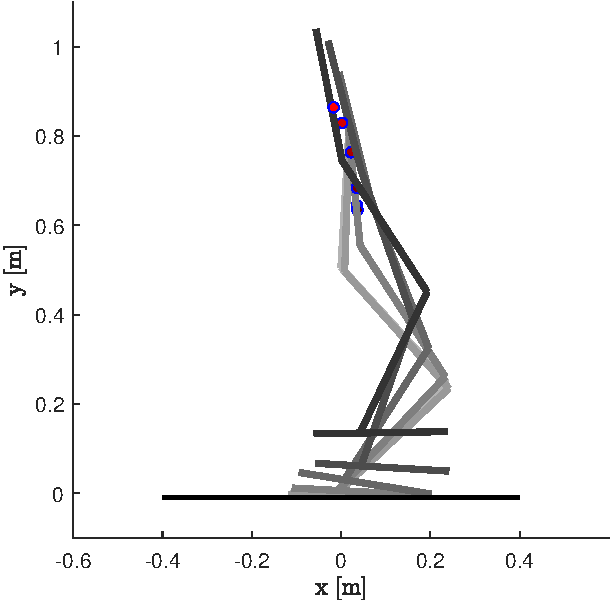
\includegraphics[scale=0.7]{initialguess}
}}
      
      \caption{Initial motion, final position in black with CoM in red}
      \label{fig:seq}
   \end{figure}
   
\section{Results} \label{sec:results}

The optimisation has been performed for the upward movement of the leg performing a jumping motion with a maximum duration of 0.4 seconds. The initial position of the leg yields a squatting posture and the optimisation is concluded when the CoM reaches its highest point for successful jumps or when the leg has fallen over for unsuccessful jumps. The initial guess is a manually constructed motion as shown in Fig. \ref{fig:seq} for actuation without energy storage branches. The optimization results for the objectives presented in Section \ref{sec:dynamicOptimisation} are shown in Tables \ref{maxheight} and \ref{minenergy}.

\begin{table}[h]
	\caption{Maximum jump height for different configurations}
	\label{maxheight}
	\begin{center}
		\begin{tabular}{c||c|c|c|c|c|c}
		\textit{Configuration}	& \textit{Height} [m] & \textit{Pretension} [m] & \textit{f} & \textit{J}$_{\text{\textit{perf.}}}$ & \textit{J}$_{\text{\textit{stab.}}}$ & \textit{J}$_{\text{\textit{torque}}}$\\
			\hline
			Only SEA &  &  &  &  &  & \\
			\hline
			Mono-articulated & &  &  &  &  &\\
			\hline
			Bi-articulated & &  &  &  &  &
		\end{tabular}
	\end{center}
\end{table}

\begin{table}[h]
	\caption{Minimum energy use for different configurations}
	\label{minenergy}
	\begin{center}
		\begin{tabular}{c||c|c|c|c|c|c}
			\textit{Configuration}	& \textit{E}$_{\text{\textit{consumed}}}$ [J] & \textit{Pretension} [m] & \textit{f} & \textit{J}$_{\text{\textit{perf.}}}$ & \textit{J}$_{\text{\textit{stab.}}}$ & \textit{J}$_{\text{\textit{torque}}}$ \\
			\hline
			Only SEA &   &   &  &  &  &\\
			\hline
			Mono-articulated &  &   &  &  &  &\\
			\hline
			Bi-articulated & &   &  &  &  &
		\end{tabular}
	\end{center}
\end{table}

\section{Discussion} \label{sec:discussion}

Comparison of actuation topologies.

\section{Conclusions} \label{sec:conclusions}

Conclusions


\addtolength{\textheight}{-12cm}   % This command serves to balance the column lengths
                                  % on the last page of the document manually. It shortens
                                  % the textheight of the last page by a suitable amount.
                                  % This command does not take effect until the next page
                                  % so it should come on the page before the last. Make
                                  % sure that you do not shorten the textheight too much.

%%%%%%%%%%%%%%%%%%%%%%%%%%%%%%%%%%%%%%%%%%%%%%%%%%%%%%%%%%%%%%%%%%%%%%%%%%%%%%%%



%%%%%%%%%%%%%%%%%%%%%%%%%%%%%%%%%%%%%%%%%%%%%%%%%%%%%%%%%%%%%%%%%%%%%%%%%%%%%%%%



%%%%%%%%%%%%%%%%%%%%%%%%%%%%%%%%%%%%%%%%%%%%%%%%%%%%%%%%%%%%%%%%%%%%%%%%%%%%%%%%


\section*{ACKNOWLEDGMENT}

Supported by European Commission projects WALK-MAN (611832), CENTAURO (644839), CoglMon (644727)


%%%%%%%%%%%%%%%%%%%%%%%%%%%%%%%%%%%%%%%%%%%%%%%%%%%%%%%%%%%%%%%%%%%%%%%%%%%%%%%%



\bibliographystyle{ieeetran}
\bibliography{lit}
\end{document}
